
%(BEGIN_QUESTION)
% Copyright 2011, Tony R. Kuphaldt, released under the Creative Commons Attribution License (v 1.0)
% This means you may do almost anything with this work of mine, so long as you give me proper credit

This Koyo ``CLICK'' PLC has been programmed to control the starting and stopping of an electric motor, including a {\it counter} instruction to prevent the motor from being started up more than a specified number of times:

$$\includegraphics[width=15.5cm]{i03589x01.eps}$$

Identify the counter instruction in the program shown, its input ``connections'', and also how the result of the counter reaching its pre-set limit forces the motor to stop.  Also, determine the maximum number of times the motor may be started up, assuming the counter's current value goes to zero when the Reset button is pressed.

\vskip 10pt

Finally, determine how to modify this PLC program so that the counter may be manually reset by the operator without requiring a separate pushbutton labeled ``Reset''.

\vskip 20pt \vbox{\hrule \hbox{\strut \vrule{} {\bf Suggestions for Socratic discussion} \vrule} \hrule}

\begin{itemize}
\item{} If an operator presses the ``Start'' button multiple times while the motor is already running, do these button-presses get counted by the counter instruction, or do only the real motor start-up events get counted?
\item{} What do you suppose the label ``CTD1'' represents inside the counter instruction?
\item{} Note the number of times the bit {\tt Y1} is referenced inside this PLC program: once in a coil instruction and twice in contact instructions.  Is there any limit to how many times a bit address may be used in a PLC program?
\item{} Describe the purpose of the first contact instruction labeled {\tt Y1} in this program, explaining why it is often referred to as a {\it seal-in} contact.
\end{itemize}

\underbar{file i03589}
%(END_QUESTION)





%(BEGIN_ANSWER)

This PLC program allows the motor to start up {\it 7} times.  If you thought the correct number of start-ups was eight, consider the fact that the counter's output bit ({\tt CT1}) gets set when the counter's current value {\it equals} the SetPoint value, not when it {\it exceeds} the SetPoint value.

\vskip 10pt

Here is a solution for an alternative Reset function:

$$\includegraphics[width=15.5cm]{i03589x02.eps}$$

In order to reset the counter, the operator must press the Stop button (after the counter has disabled the system from starting).

%(END_ANSWER)





%(BEGIN_NOTES)



\vskip 20pt \vbox{\hrule \hbox{\strut \vrule{} {\bf Virtual Troubleshooting} \vrule} \hrule}

This question is a good candidate for a ``Virtual Troubleshooting'' exercise.  Presenting the diagram to students, you first imagine in your own mind a particular fault in the system.  Then, you present one or more symptoms of that fault (something noticeable by an operator or other user of the system).  Students then propose various diagnostic tests to perform on this system to identify the nature and location of the fault, as though they were technicians trying to troubleshoot the problem.  Your job is to tell them what the result(s) would be for each of the proposed diagnostic tests, documenting those results where all the students can see.

During and after the exercise, it is good to ask students follow-up questions such as:

\begin{itemize}
\item{} What does the result of the last diagnostic test tell you about the fault?
\item{} Suppose the results of the last diagnostic test were different.  What then would that result tell you about the fault?
\item{} Is the last diagnostic test the best one we could do?
\item{} What would be the ideal order of tests, to diagnose the problem in as few steps as possible?
\end{itemize}


%INDEX% PLC, ladder logic program analysis and explanation (Koyo CLICK)

%(END_NOTES)


